\documentclass[12pt]{article}

\usepackage[utf8]{inputenc}
\usepackage{latexsym,amsfonts,amssymb,amsthm,amsmath}
\usepackage{tikz}
\usepackage{stanli}
\usetikzlibrary{shapes,calc,through,3d,patterns}
\usetikzlibrary{arrows.meta,decorations.pathreplacing,angles,quotes}
\usepackage{multicol}
\usepackage{geometry}
\usepackage{mathtools}
\usepackage{siunitx}
\usepackage{booktabs}

\setlength{\parindent}{0in}
\setlength{\oddsidemargin}{-0.25in}
\setlength{\textwidth}{7in}
\setlength{\textheight}{9.3in}
\setlength{\topmargin}{-1in}
\setlength{\headheight}{18pt}

\newcommand\blfootnote[1]{%
    \begingroup
    \renewcommand\thefootnote{}\footnote{#1}%
    \addtocounter{footnote}{-1}%
    \endgroup
}

\definecolor{darkred}{rgb}{0.6,0,0}

\newcommand{\bolddelta}{\boldsymbol\delta}
\newcommand{\boldxi}{\boldsymbol\xi}

\begin{document}

\noindent ME473 - Dynamic finite element analysis of structures\hfill EPFL\\
Stefano Burzio \hfill 2025\\
\vspace{0.3cm}

\hspace*{\fill}\textbf{\Large Problem set 4 - solutions}\hspace*{\fill}

\hrulefill

\subsection*{Problem 1}
To derive the weak form, we multiply the governing equation by a virtual temperature (test function) \( \delta T \) and integrate over the domain \(\Omega\):

\[
    \int_{\Omega} \rho c \frac{\partial T}{\partial t} \delta T \, d\Omega = \int_{\Omega} \left[ \text{div}(k \nabla T) + f_0 \right] \delta T \, d\Omega.
\]

Then, we apply the divergence theorem to the divergence term:

\[
    \int_{\Omega} \text{div}(k \nabla T) \delta T \, d\Omega = - \int_{\Omega} k \nabla T \cdot \nabla\delta T \, d\Omega + \int_{\partial \Omega} k \nabla T \cdot \hat{n} \delta T \, d\Gamma.
\]

Recall that $\nabla T \cdot \hat{n}=\frac{\partial T}{\partial \hat{n}}$ represents the directional derivative of $T$ in the outward normal direction to the boundary. Since for the virtual temperature \(\delta T = 0\) on the boundary \(\partial \Omega\), the boundary term vanishes, and we obtain:

\begin{eqnarray}
    \label{eq:wf}
    \int_{\Omega} \rho c \frac{\partial T}{\partial t}\delta T \, d\Omega + \int_{\Omega} k \nabla T \cdot \nabla \delta T \, d\Omega = \int_{\Omega} f_0 \delta T \, d\Omega.
\end{eqnarray}

We approximate the real and virtual temperatures using finite element basis functions \( h_i \) and nodal values \( q_i(t) \) for $i=1,\dots,6$:
\[
    T^h(x, y, t) \approx \sum_{i=1}^{6} q_i(t) h_i(x, y)\qquad \text{and}\qquad \delta T^h(x, y) \approx \sum_{j=1}^{6} \delta q_j h_j(x, y).
\]

Substituting this into the weak form \eqref{eq:wf} leads us to

\[
    \sum_{i=1}^{6} \sum_{j=1}^{6} \delta q_j\Big(\int_{\Omega} \rho c  h_i h_j \, d\Omega\ \dot{q}_i(t) + \int_{\Omega} k (\nabla h_i)^T \nabla h_j \, d\Omega\ q_i(t)\Big)= \sum_{j=1}^{6} \delta q_j \int_{\Omega} f_0  h_j \, d\Omega
\]

The semi-discrete weak form results in the following system of ordinary differential equations for the nodal temperatures \( q_i(t) \):

\[
    \mathbf{M} \mathbf{\dot{q}}+  \mathbf{K} \mathbf{q} = \mathbf{r}
\]
where:
\begin{itemize}
    \item \(\mathbf{q}\) is the vector of unknown nodal temperatures \( q_i(t)\),
    \item \(\mathbf{M}\) is the heat capacity (or capacitance) matrix with components:
          $
              m_{ij} = \int_{\Omega} \rho c h_i h_j \, d\Omega,
          $
    \item  \(\mathbf{K}\) is the thermal conductivity matrix with components:
          $
              k_{ij} = \int_{\Omega} k (\nabla h_i)^T \nabla h_j \, d\Omega,
          $
    \item  \(\mathbf{r}\) is heat source vector with components:
          $
              r_i = \int_{\Omega} f_0 h_i \, d\Omega.
          $
\end{itemize}
The following code, available on the \texttt{MATLAB} drive, solves a transient heat conduction problem. The code defines the material properties, generates a mesh, computes elementary thermal conductivity and heat capacity matrices and elementary heat source vector, assembles them into global matrices, applies boundary conditions, and solves the system. The script is structured as follows:
\begin{itemize}
    \item Define material properties and mesh parameters.
    \item Compute elementary matrices and vectors using the archetypal triangular element.
    \item Assemble the global system.
    \item Apply boundary conditions and solve the system using an ODE solver.
    \item Visualize the temperature distribution over time.
\end{itemize}

\subsubsection*{Define material properties and mesh parameters}
The first section of the code defines the physical properties of the material being analyzed, such as density, thermal conductivity, and specific heat capacity. It also specifies the geometry and mesh, which includes defining the node positions and element connectivity. These parameters are essential for setting up the finite element model.

\begin{verbatim}
clear 
clc
%% Parameters
rho = 2700;   % Density of aluminum (kg/m^3)
c = 900;      % Specific heat capacity (J/kg.K)
k = 205;      % Thermal conductivity (W/m.K)
f0 = 1e6;     % Heat source (W/m^2)
a = 0.1;      % Radius of the circular plate (m)
t_final = 20; % Total simulation time (s)

% Nodes coordinates
number_nodes = 6;
x1 = [0, a/2, a, a/(2*sqrt(2)), a*cos(pi/8),a/(sqrt(2))];
y1 = [0, 0, 0, a/(2*sqrt(2)), a*sin(pi/8), a/(sqrt(2))];

nodes_coord = transpose([x1; y1]);

% Plot nodes 
plot_nodes(nodes_coord)
\end{verbatim}
\begin{center}
    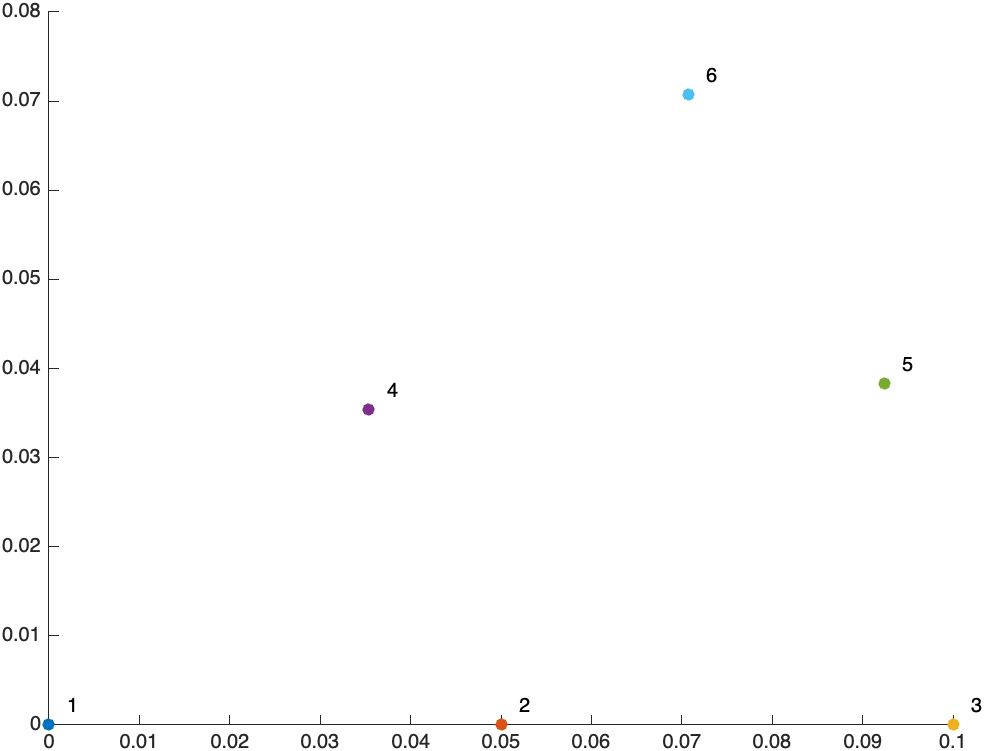
\includegraphics[width=8cm]{../images/nodes_trg.png}
\end{center}

Next, we define the local shape functions for a bilinear 2D triangular finite element  and establish a connectivity matrix for a simple finite element mesh with four elements. The connectivity matrix proposed here is not unique, and may vary depending on the chosen node numbering within each element. However, it is important to note that while different connectivity choices may lead to different local matrices and vectors, the global matrices and vectors must remain invariant to the connectivity choice in order to ensure consistency in the finite element analysis.

\begin{verbatim}
% Local shape functions
syms xi1 xi2
Ha(1) = 1 - xi1 - xi2;
Ha(2) = xi1;
Ha(3) = xi2;

% Connectivity matrix
number_elements = 4;
connectivity = cell(1, number_elements); 

connectivity{1} = [1; 2; 4];
connectivity{2} = [2; 3; 5];
connectivity{3} = [2; 5; 4];
connectivity{4} = [4; 5; 6];
\end{verbatim}

\subsubsection*{Compute elementary matrices and vectors}
This code computes the Jacobian matrix, its inverse, and determinant for each element in a finite element model. Then it loops over all elements, calculating elementary thermal conductivity and heat capacity matrices and the heat source vector.
\begin{verbatim}    
% Compute Jacobian
transf = cell(1, number_elements); 
jac_mat = cell(1, number_elements); 
jac_inv = cell(1, number_elements); 
jac_det = cell(1, number_elements); 
    
for e = 1:number_elements
    local_nodes_indices = connectivity{e};
    transf{e} = simplify(Ha * nodes_coord(local_nodes,:));
    jac_mat{e} = jacobian(transf{e}, [xi1, xi2]);
    jac_det{e} = det(jac_mat{e});
    jac_inv{e} = inv(jac_mat{e});
end
    
plot_trg_elements(transf, xi1, xi2,number_elements,'blue', '.');
\end{verbatim}
\begin{center}
    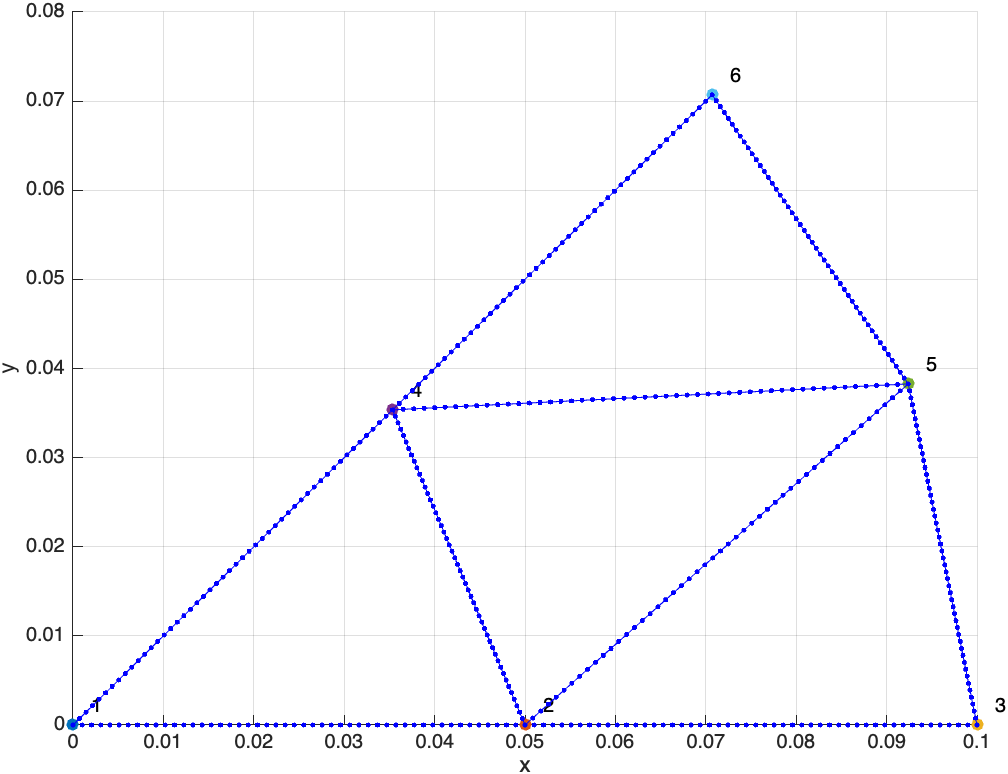
\includegraphics[width=8cm]{../images/elem_trg.png}
\end{center}
\begin{verbatim}
% Elementary thermal conductivity and heat capacity matrices and heat source vector  
K_elem = cell(1, number_elements);
M_elem = cell(1, number_elements);
r_elem = cell(1, number_elements);
    
Ba = simplify([diff(Ha,xi1); diff(Ha,xi2)]);
    
for e=1:number_elements
    K_elem{e} = int(int(k * transpose(jac_inv{e}*Ba)*jac_inv{e}*Ba*jac_det{e},
                    xi2,[0,1-xi1]),xi1,[0,1]);
    M_elem{e} = int(int(rho * c * transpose(Ha) * Ha  * jac_det{e},
                    xi2,[0,1-xi1]),xi1,[0,1]);
    r_elem{e} = int(int(f0 * transpose(Ha) * jac_det{e},xi2,[0,1-xi1]),xi1,[0,1]);
end
\end{verbatim}

\subsubsection*{Assemble the global system}
After computing the elementary matrices, they are assembled into global matrices, representing the entire domain's behavior. This step involves summing contributions from each element into larger matrices that describe the entire system's thermal response.
\begin{verbatim}    
% Global thermal conductivity and heat capacity matrices and heat source vector 
K_global = zeros(number_nodes);
M_global = zeros(number_nodes);
r_global = zeros(number_nodes);
    
for e=1:number_elements
    indices = connectivity{e};
    K_global(indices,indices) = K_global(indices,indices) + K_elem{e};
    M_global(indices,indices) = M_global(indices,indices) + M_elem{e};
    r_global(indices) = r_global(indices) + r_elem{e};
end    
\end{verbatim}

\subsubsection*{Apply boundary conditions and solve the system using an ODE solver}
The code applies boundary conditions by identifying constrained nodes and modifying the global system accordingly. The system is then solved using an ODE solver (ode45) to compute the transient temperature evolution over time.
\begin{verbatim}    
% Boundary conditions
constrained_nodes = [3 5 6]; % nodes that have prescribed degree of freedom
given_values_at_constrained_nodes = [0 0 0]; 
    
indices_free_nodes = setdiff((1:number_nodes)',constrained_nodes);

K_global_free_nodes = K_global(indices_free_nodes, indices_free_nodes);
M_global_free_nodes = M_global(indices_free_nodes, indices_free_nodes);
r_global_free_nodes = r_global(indices_free_nodes);
    
% Compute the inverse of the heat capacity matrix
M_inv = inv(M_global_free_nodes);
    
% Define the system of ODEs
ode_fun = @(t, q) M_inv * (r_global_free_nodes - K_global_free_nodes * q);
    
% Initial condition (assuming initial temperature is zero at free nodes)
q0 = zeros(length(indices_free_nodes), 1);
    
% Time span for the simulation
tspan = [0 t_final];
    
% Solve the system using ode45 (or use ode15s if it's stiff)
[t_sol, q_sol] = ode45(ode_fun, tspan, q0);
    
for i = 1:length(t_sol)
    % Assign free nodes' temperatures
    q_full(indices_free_nodes, i) = q_sol(i, :)'; 
    % Assign fixed values
    q_full(constrained_nodes, i) = given_values_at_constrained_nodes; 
end
\end{verbatim}

\subsubsection*{Visualize the temperature distribution over time}
Finally, the results are visualized using a trisurf plot, which displays the temperature distribution over the domain. The visualization updates at different time steps to show how heat propagates through the material.
\begin{verbatim}  
% Plot temperature evolution at selected time steps
tri = [connectivity{1}'; connectivity{2}'; connectivity{3}'; connectivity{4}'];

% Plot temperature evolution as a surface
figure;
for i = 1:5:length(t_sol)
    clf;
    trisurf(tri, nodes_coord(:,1), nodes_coord(:,2), q_full(:,i), 'FaceColor', 'interp');
    colorbar;
    caxis([min(q_full(:)) max(q_full(:))]); % Keep consistent color scale
    shading interp;
    title(sprintf('Temperature Distribution at t = %.2f s', t_sol(i)));
    xlabel('X Position (m)');
    ylabel('Y Position (m)');
    view(2); % Top-down view
    axis equal;
    pause(1); % Pause to create an animation effect
end  
\end{verbatim}
\begin{center}
    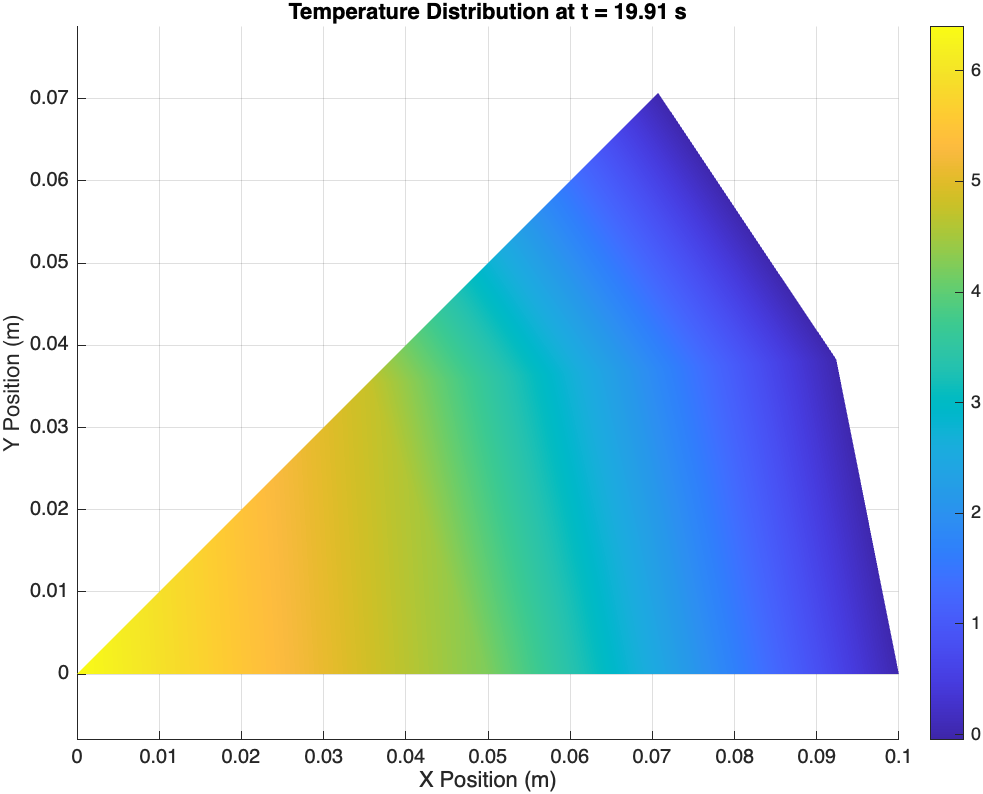
\includegraphics[width=10cm]{../images/temp_trg.png}
\end{center}
\end{document}